%%%%%%%%%%%%%%%%%%%%%%%%%%%%%%%%%%%%%%%%%%%%%%%%%%%%%%%%%%%%%%%%%%%%%%%%%%%%%%%%%%
\begin{frame}[fragile]\frametitle{}
\begin{center}
{\Large Deep Learning Frameworks}
\end{center}
\end{frame}


% %%%%%%%%%%%%%%%%%%%%%%%%%%%%%%%%%%%%%%%%%%%%%%%%%%%
% \begin{frame}[fragile] \frametitle{Implementation of neural networks}
% \begin{itemize}

% \item Think of neural networks as being primarily
% defined by a network of individual neurons. 
% \item Helpful both for its simplicity and the historical development of the
% estimators. 
% \item There is a closer way that mimics popular implementations
% such as Caffe, Keras, Torch and TensorFlow.
% \end{itemize}
% \end{frame}


%%%%%%%%%%%%%%%%%%%%%%%%%%%%%%%%%%%%%%%%%%%%%%%%%%%
\begin{frame}[fragile] \frametitle{Neural network software / libraries}
\begin{itemize}
\item Many libraries have been written for training
classes of neural networks. 
\item Most of these try to support operations being compiled to a GPU.
\item Data preprocessing, modeling network, evaluating output, graphical debugging, are some of the facilities given by these libraries.
\end{itemize}
\end{frame}

%%%%%%%%%%%%%%%%%%%%%%%%%%%%%%%%%%%%%%%%%%%%%%%%%%%
\begin{frame}[fragile] \frametitle{}


\includegraphics[width=0.8\linewidth]{torch.pdf}

\end{frame}

%%%%%%%%%%%%%%%%%%%%%%%%%%%%%%%%%%%%%%%%%%%%%%%%%%%
\begin{frame}[fragile] \frametitle{}

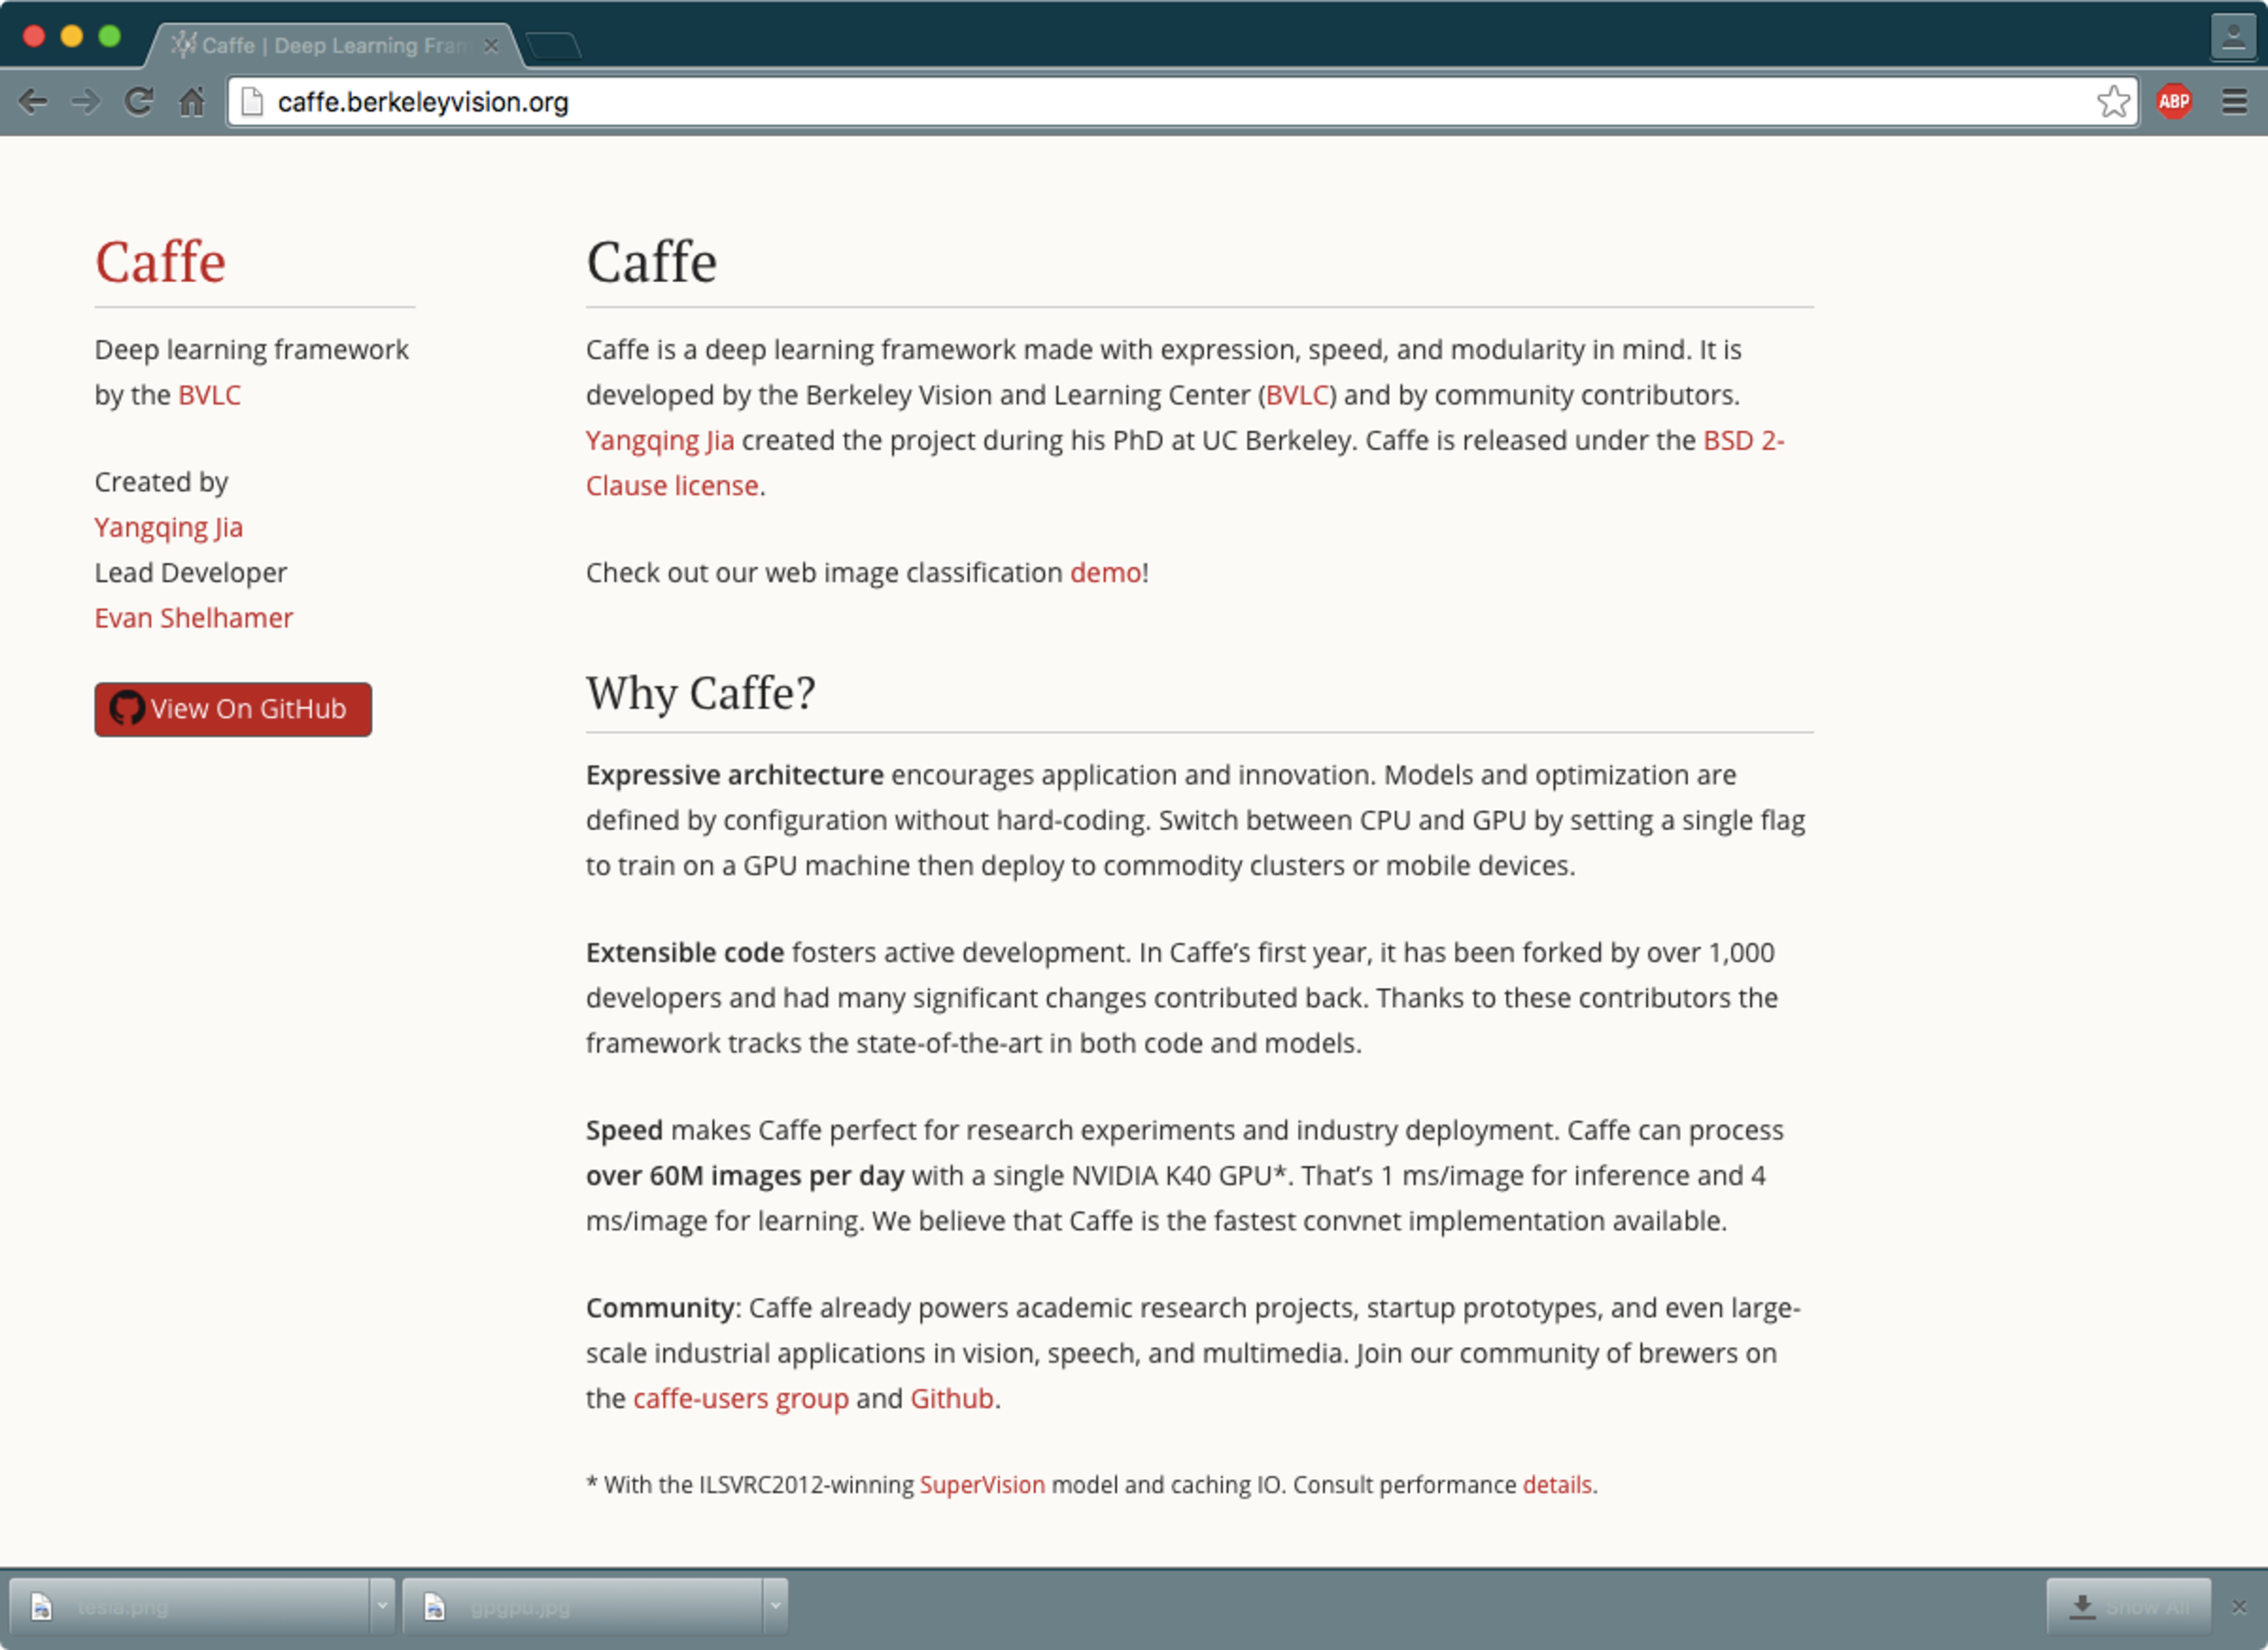
\includegraphics[width=0.8\linewidth]{caffee.pdf}

\end{frame}

% %%%%%%%%%%%%%%%%%%%%%%%%%%%%%%%%%%%%%%%%%%%%%%%%%%%
% \begin{frame}[fragile] \frametitle{}

% 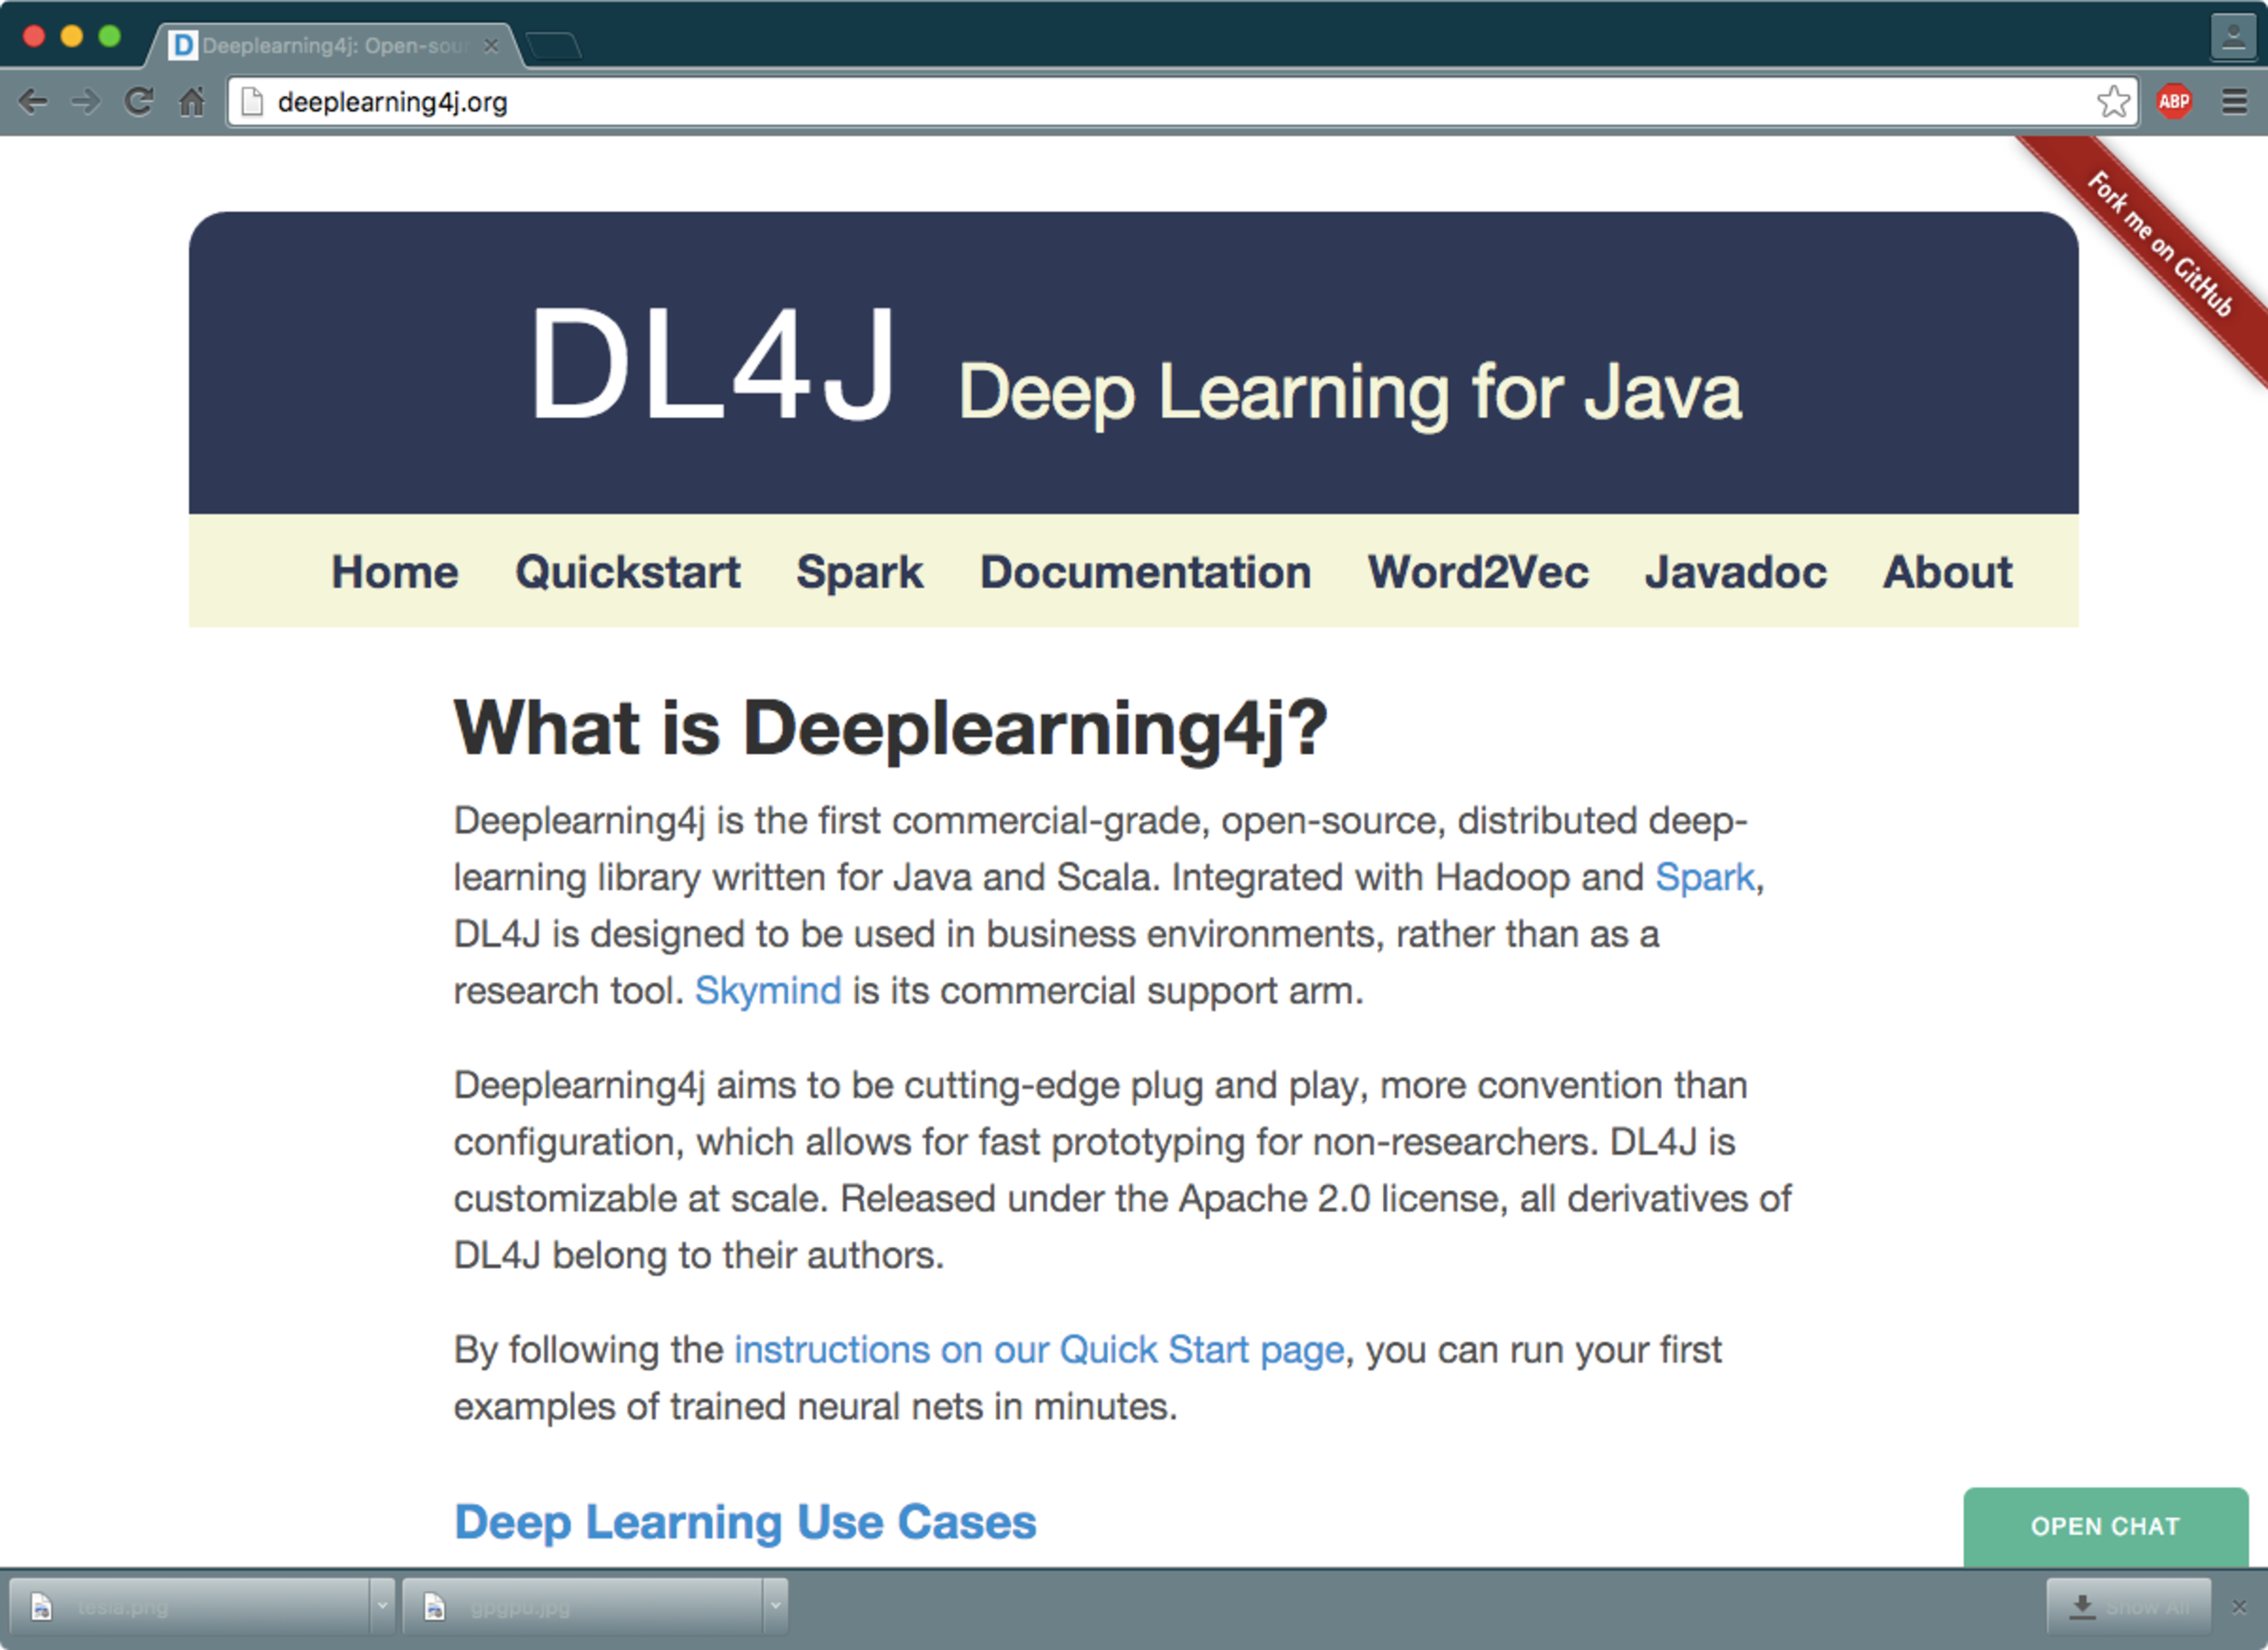
\includegraphics[width=0.8\linewidth]{deeplearning.pdf}

% \end{frame}

% %%%%%%%%%%%%%%%%%%%%%%%%%%%%%%%%%%%%%%%%%%%%%%%%%%%
% \begin{frame}[fragile] \frametitle{}

% 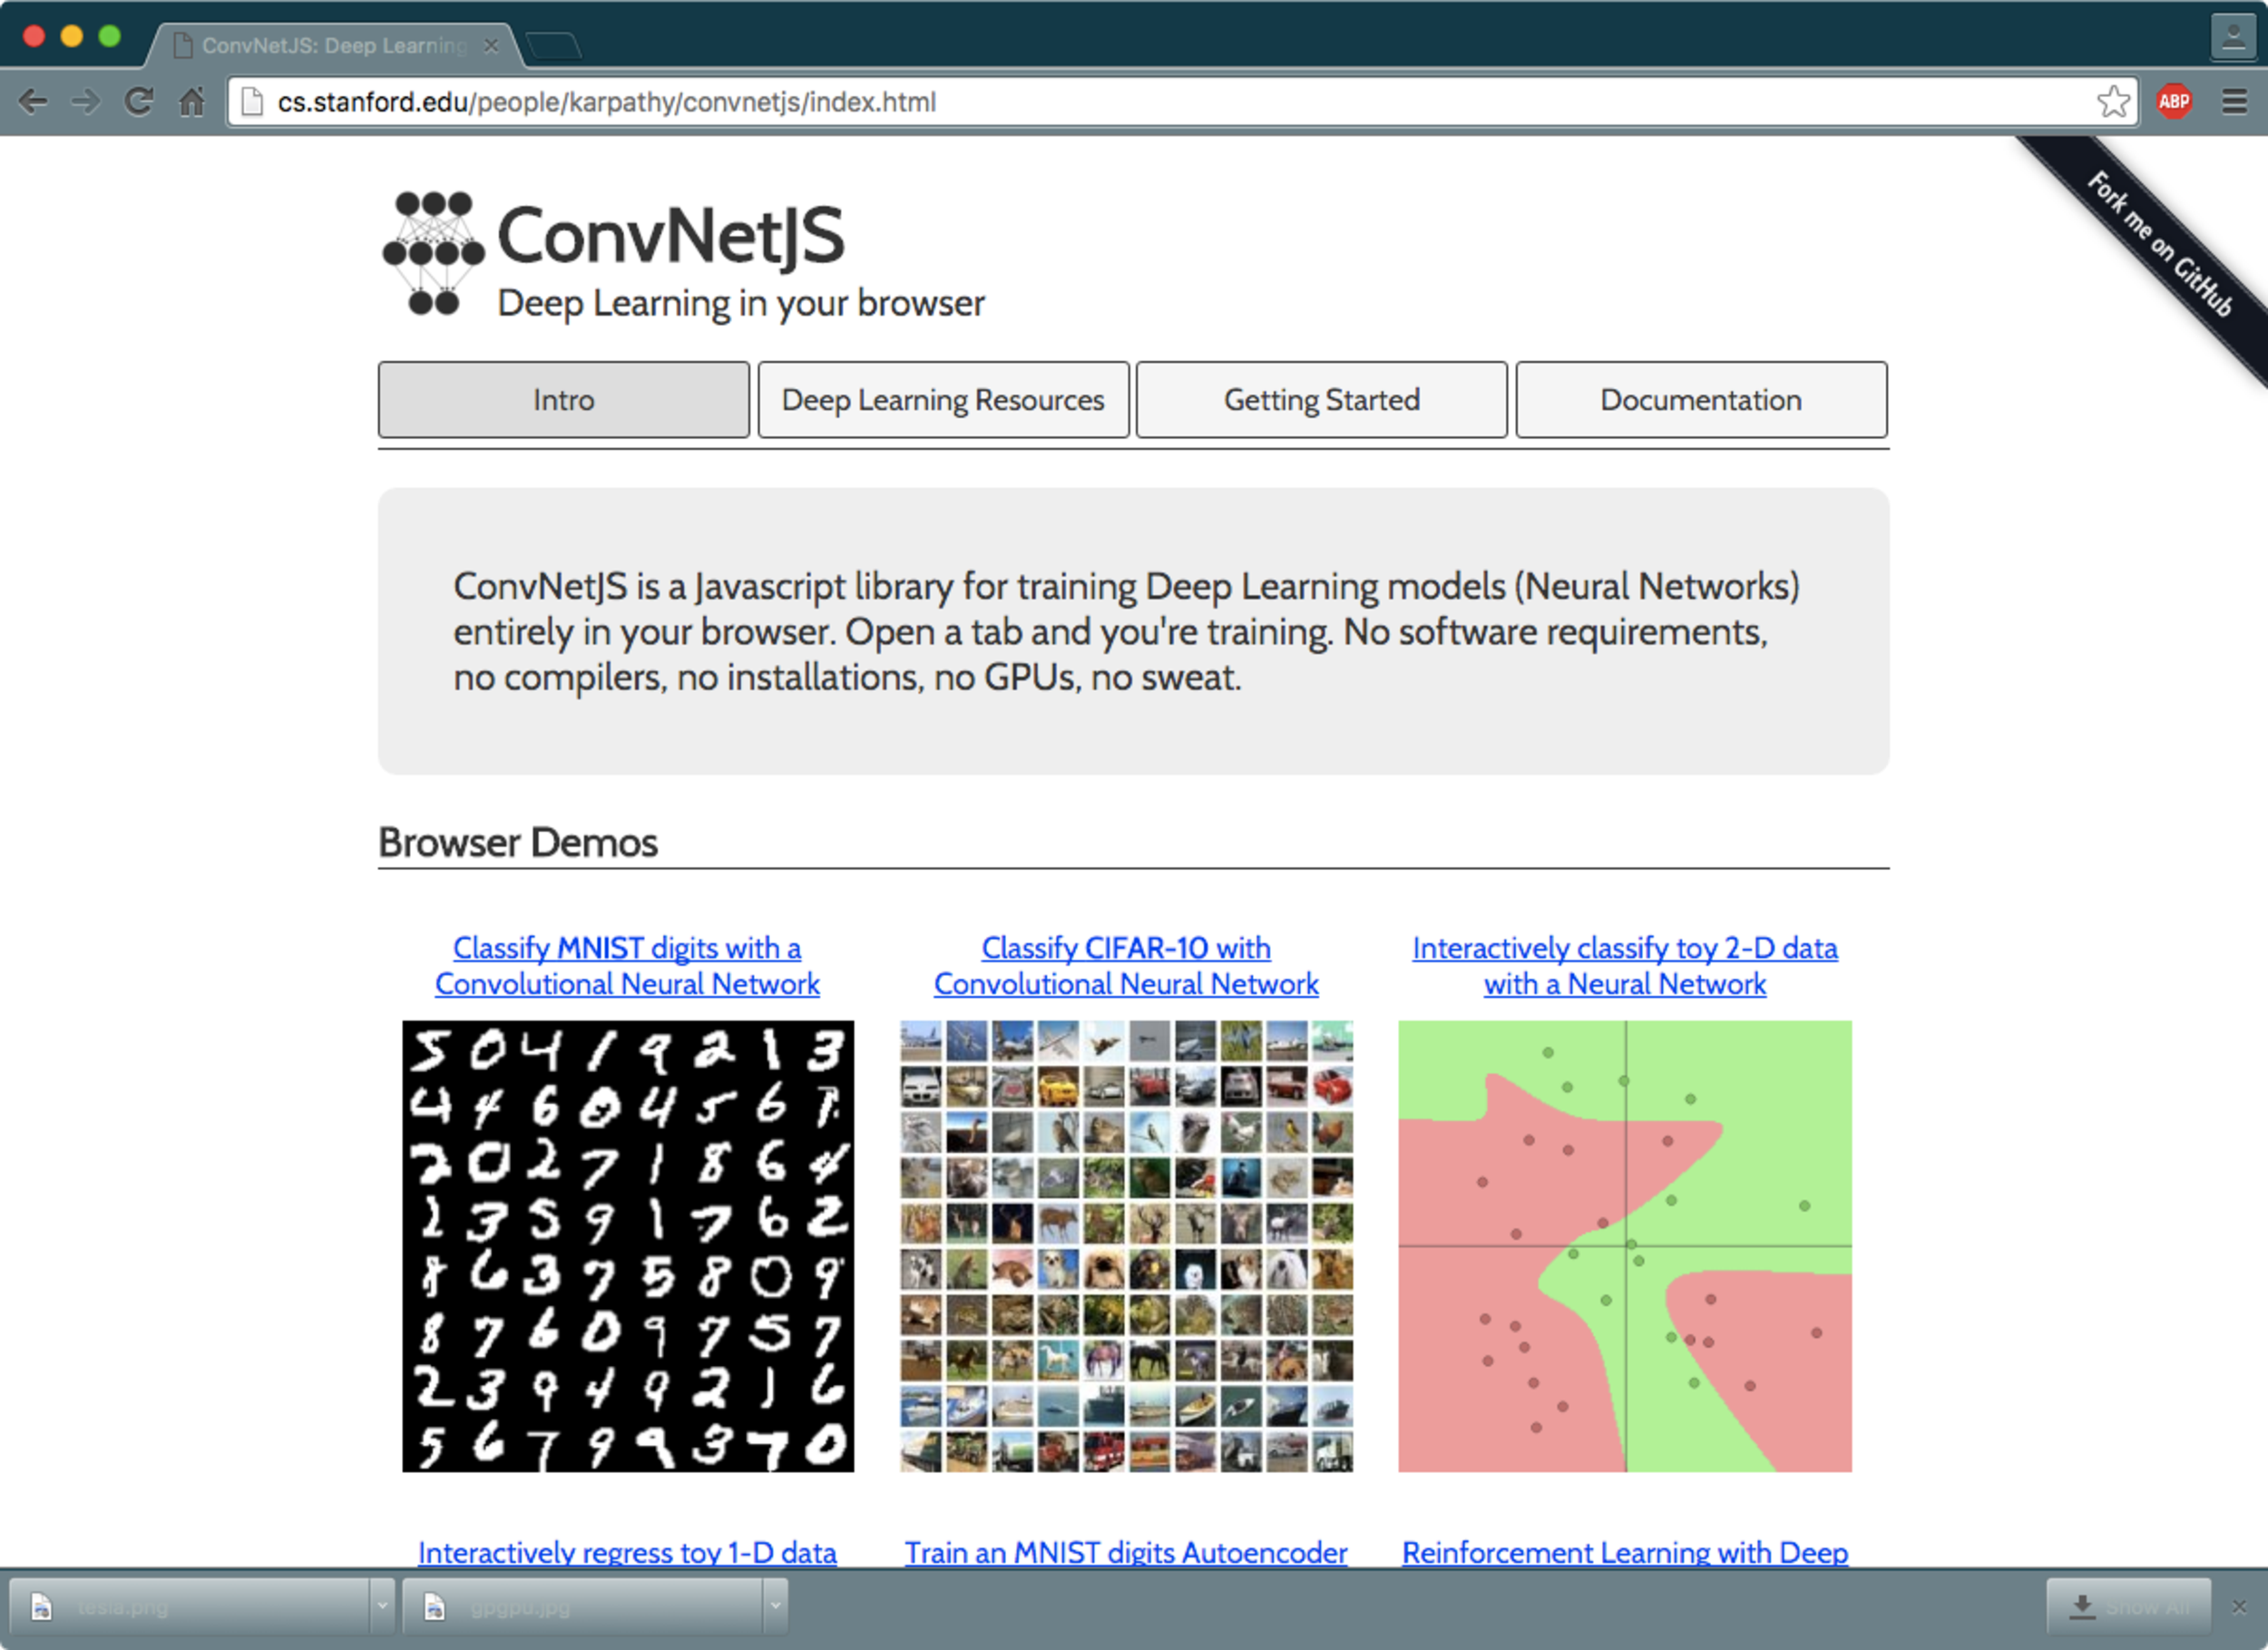
\includegraphics[width=0.8\linewidth]{convnetjs.pdf}

% \end{frame}

%%%%%%%%%%%%%%%%%%%%%%%%%%%%%%%%%%%%%%%%%%%%%%%%%%%
\begin{frame}[fragile] \frametitle{}

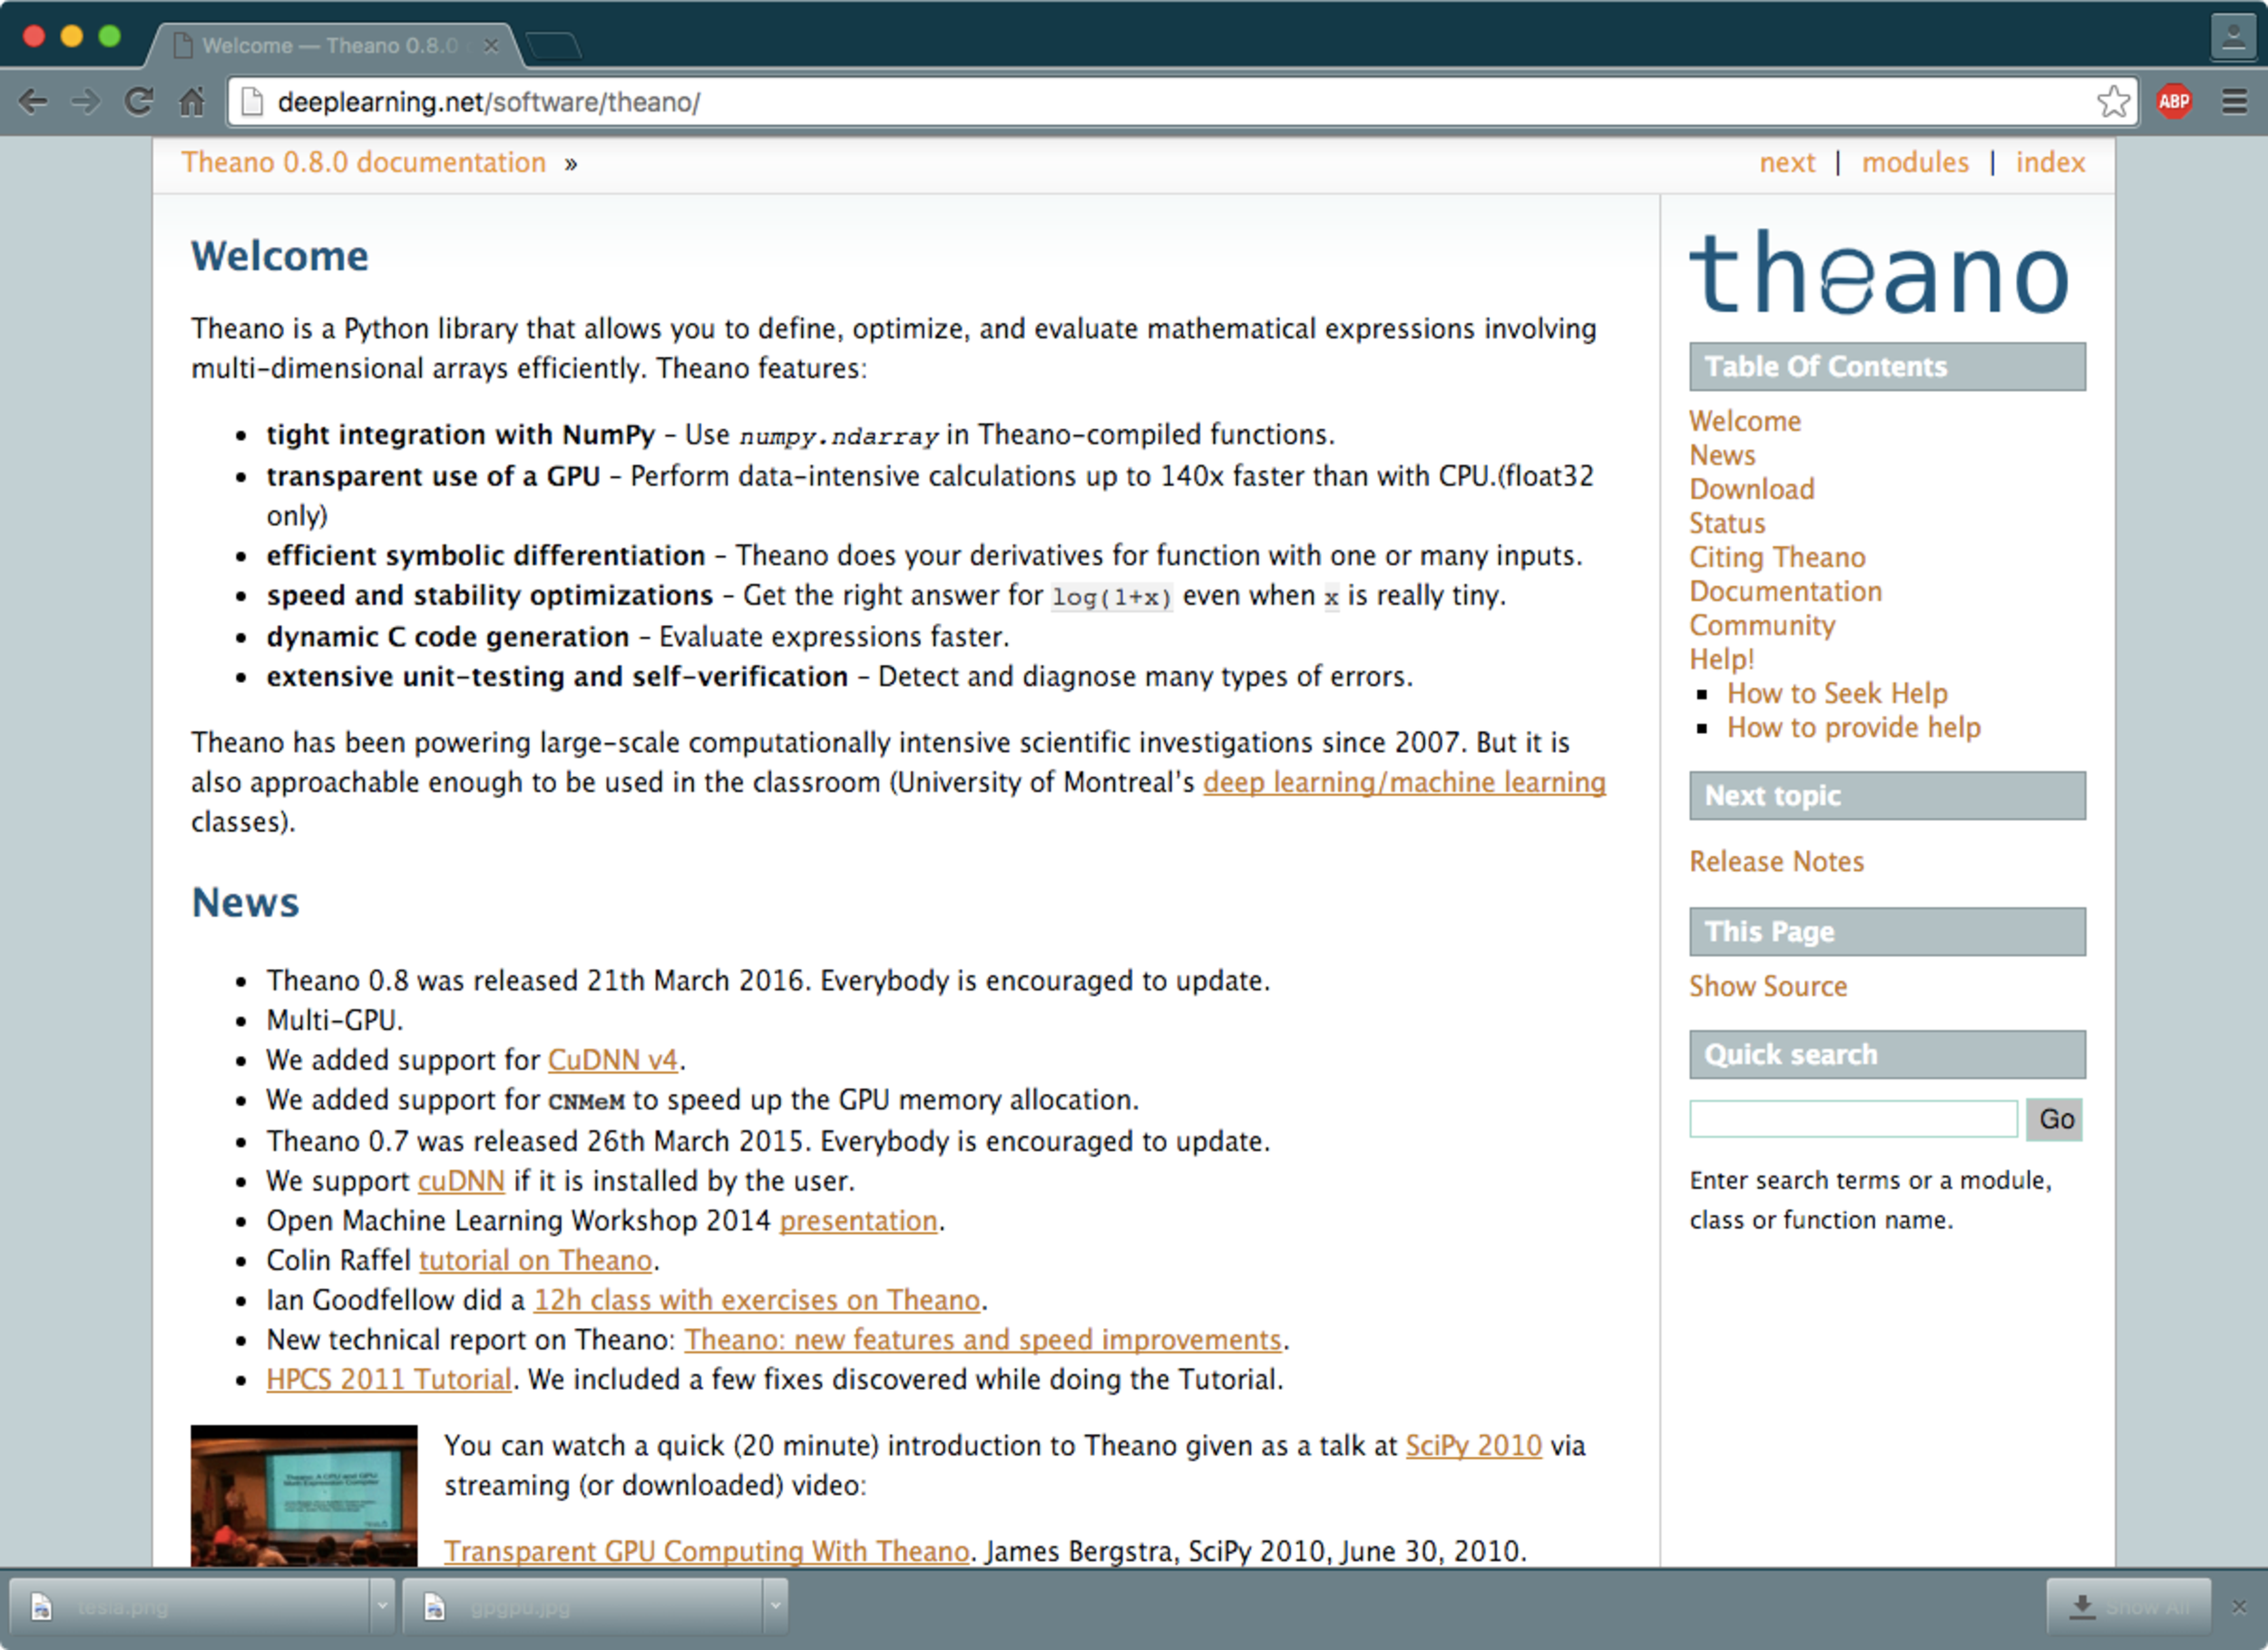
\includegraphics[width=0.8\linewidth]{theano.pdf}

\end{frame}

%%%%%%%%%%%%%%%%%%%%%%%%%%%%%%%%%%%%%%%%%%%%%%%%%%%
\begin{frame}[fragile] \frametitle{}

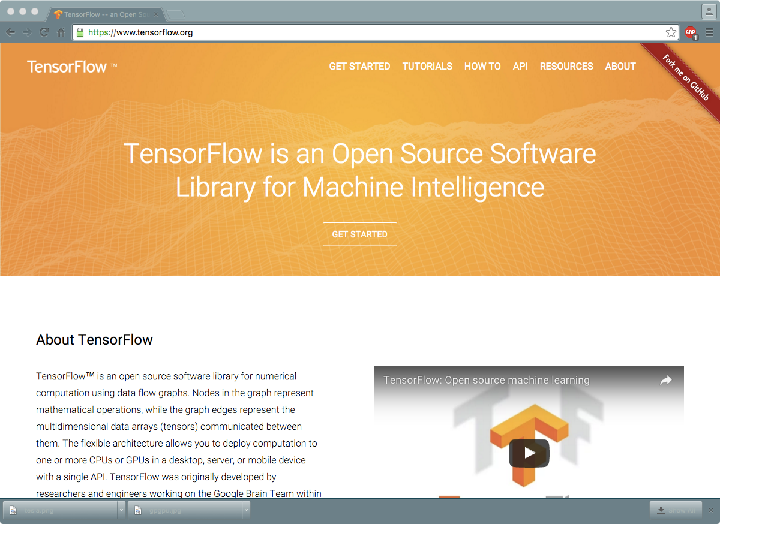
\includegraphics[width=0.8\linewidth]{tensorflow}

\end{frame}

% %%%%%%%%%%%%%%%%%%%%%%%%%%%%%%%%%%%%%%%%%%%%%%%%%%%
% \begin{frame}[fragile] \frametitle{}

% 
\includegraphics[width=0.8\linewidth]{blocks.pdf}

% \end{frame}

% %%%%%%%%%%%%%%%%%%%%%%%%%%%%%%%%%%%%%%%%%%%%%%%%%%%
% \begin{frame}[fragile] \frametitle{}

% 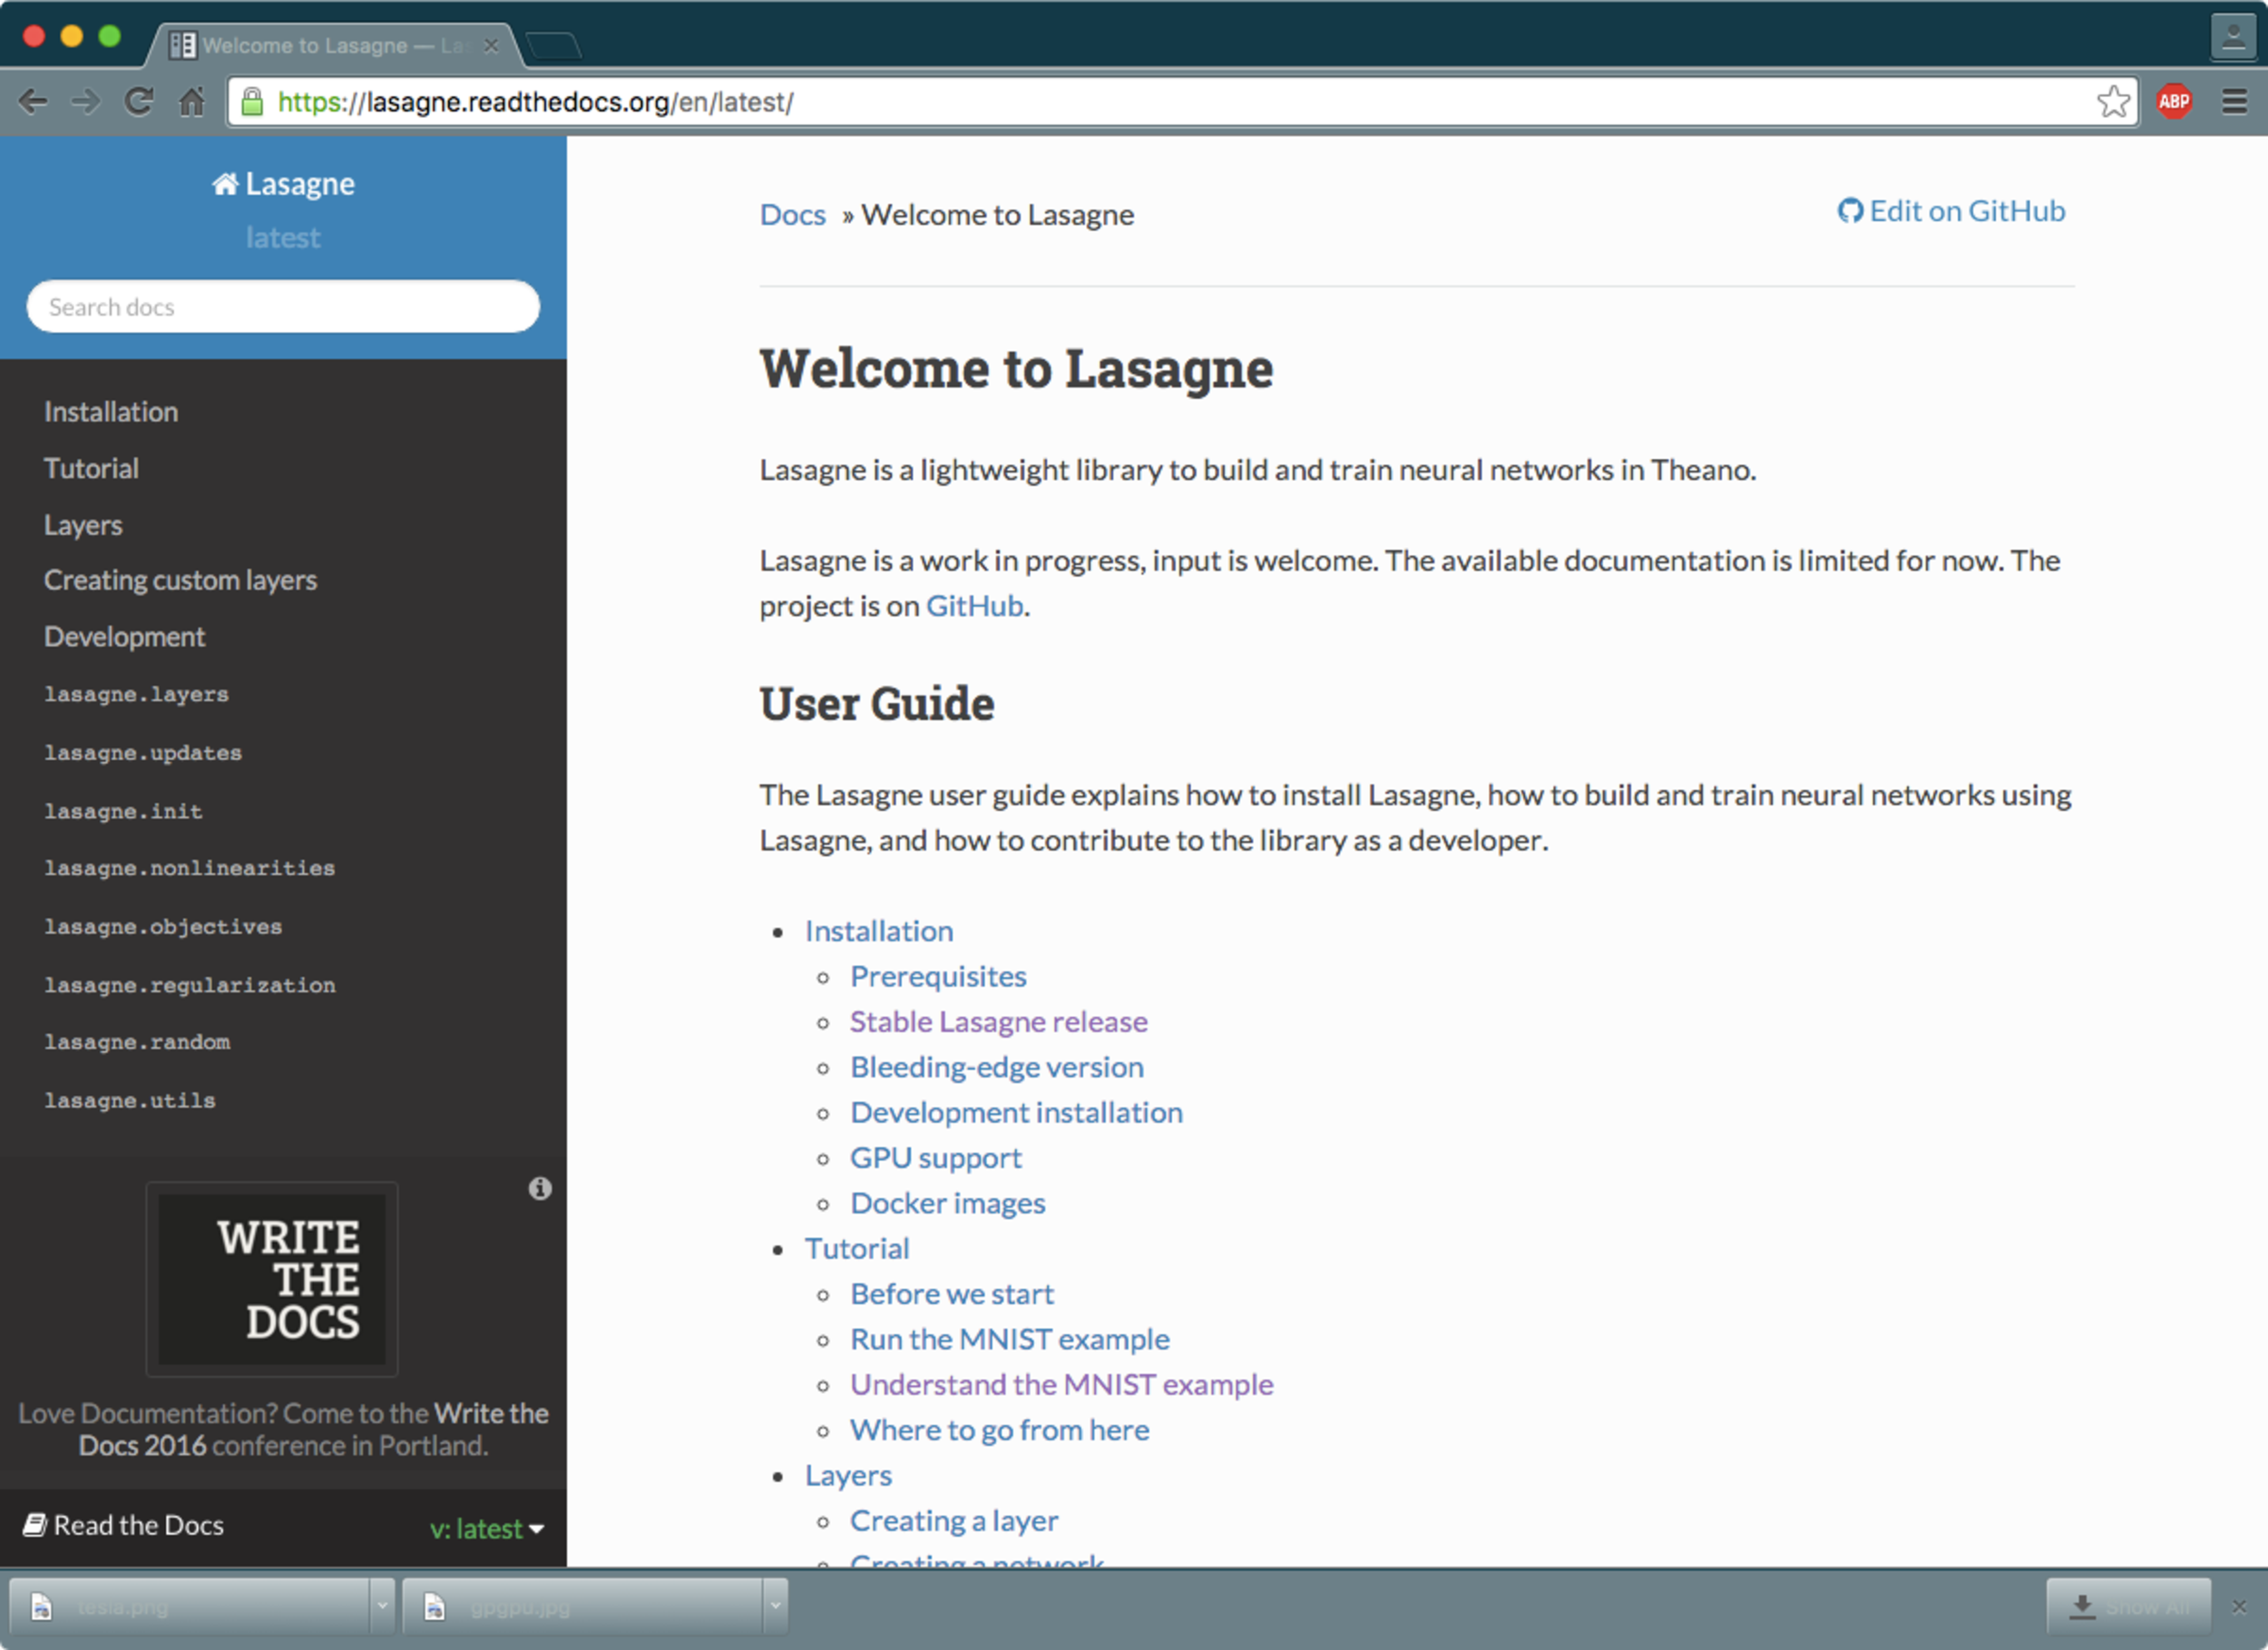
\includegraphics[width=0.8\linewidth]{lasagna.pdf}

% \end{frame}

%%%%%%%%%%%%%%%%%%%%%%%%%%%%%%%%%%%%%%%%%%%%%%%%%%%
\begin{frame}[fragile] \frametitle{}

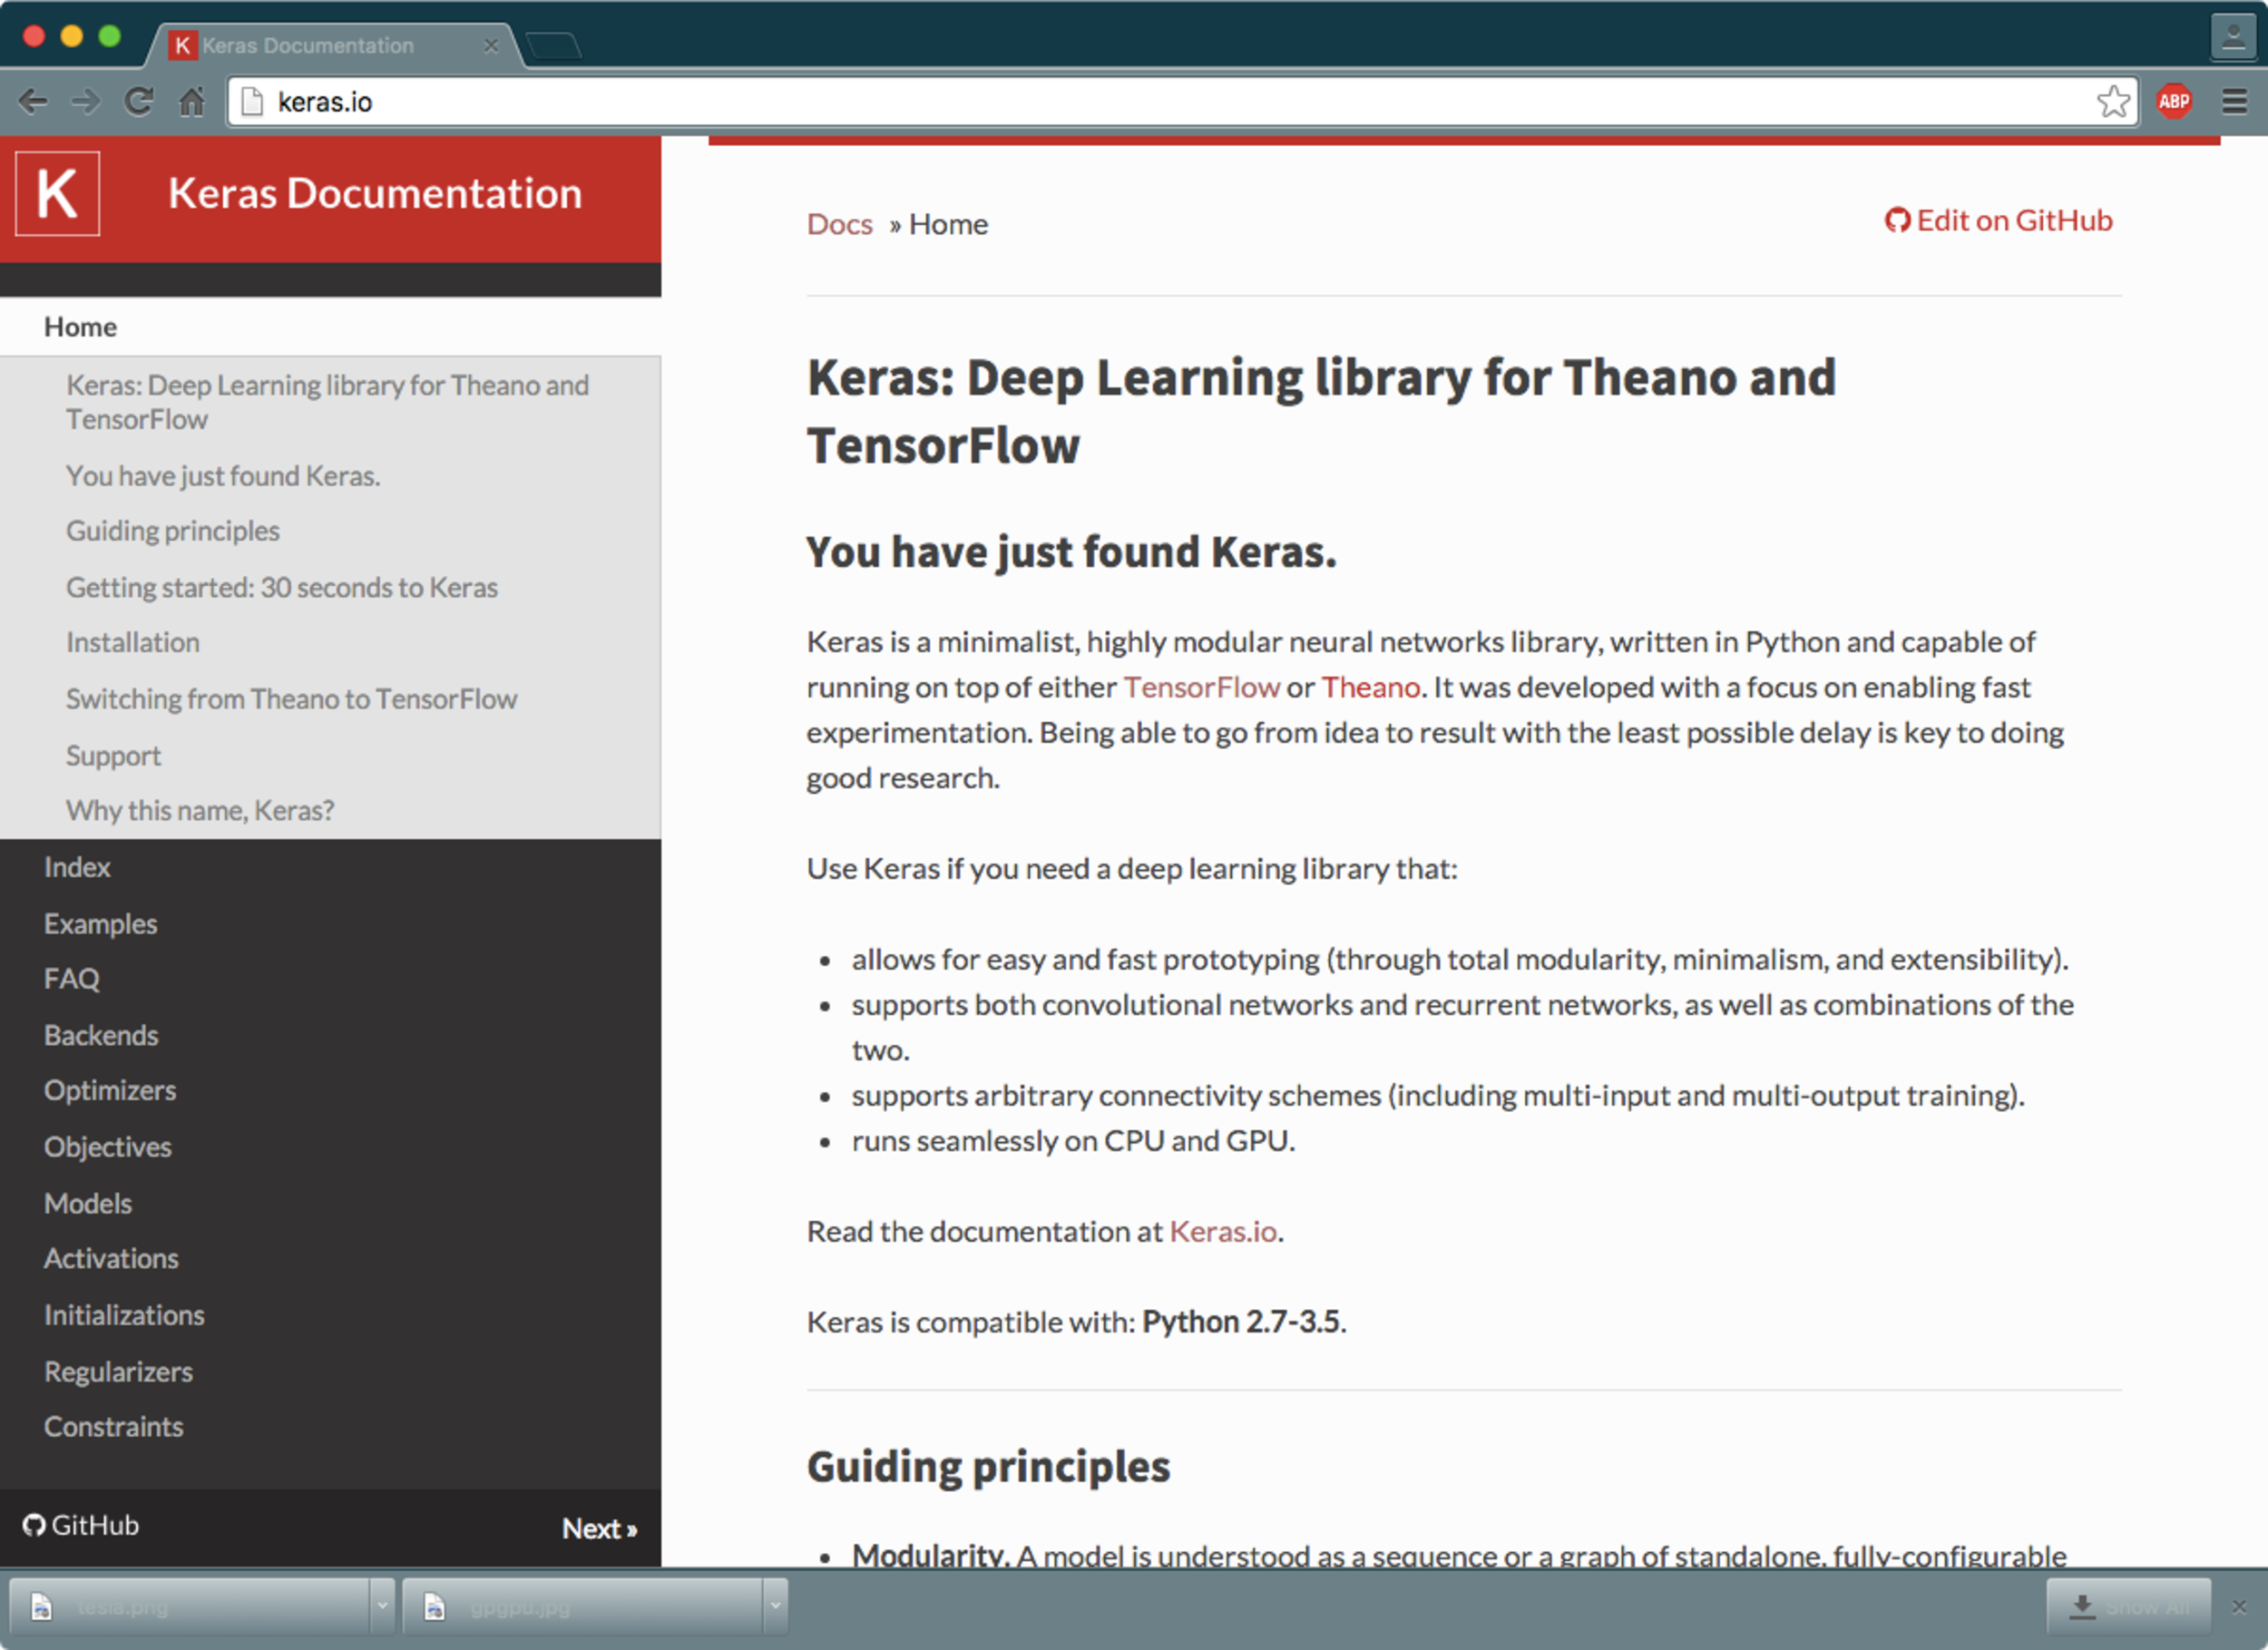
\includegraphics[width=0.8\linewidth]{keras.pdf}

\end{frame}

% %%%%%%%%%%%%%%%%%%%%%%%%%%%%%%%%%%%%%%%%%%%%%%%%%%%
% \begin{frame}[fragile] \frametitle{Hardware Role}

% \begin{itemize}

% \item Many of the layers consist of applying
% tensor/matrix products. 
% \item Need highly optimized libraries, often written to take special
% advantage of the particular architecture of a given CPU/GPU.

% \begin{center}
% 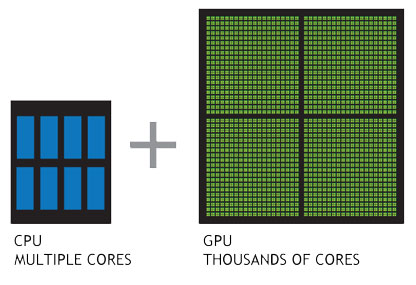
\includegraphics[width=0.5\linewidth,keepaspectratio]{gpgpu.jpg}
% \end{center}

% \end{itemize}
% \end{frame}

% %%%%%%%%%%%%%%%%%%%%%%%%%%%%%%%%%%%%%%%%%%%%%%%%%%%
% \begin{frame}[fragile] \frametitle{Example: NVIDIA Tesla}

% These are now virtually required for doing cutting-edge neural network
% research:

% \begin{center}
% 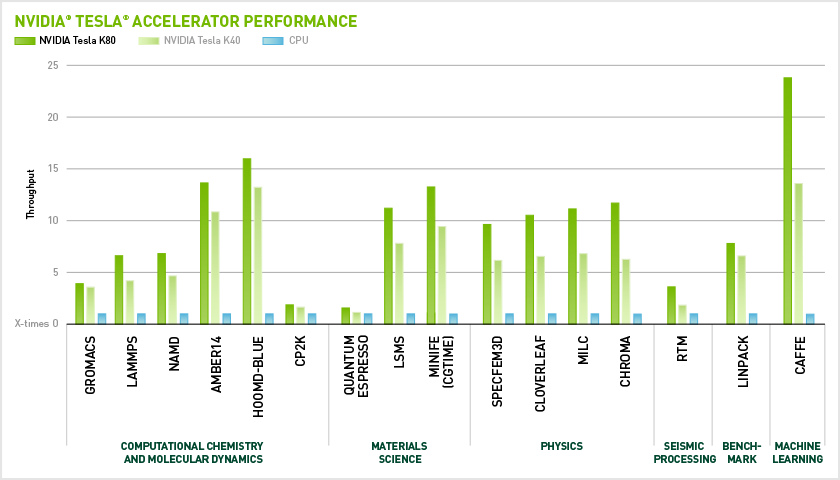
\includegraphics[width=0.8\linewidth,keepaspectratio]{tesla.png}
% \end{center}

% \end{frame}


